% -*- TeX-engine: xetex; eval: (auto-fill-mode 0); eval: (visual-line-mode 1); -*-
% Compile with XeLaTeX

%%%%%%%%%%%%%%%%%%%%%%%
% Option 1: Slides: (comment for handouts)   %
%%%%%%%%%%%%%%%%%%%%%%%
\documentclass[slidestop,compress,mathserif,11pt,t,professionalfonts,xcolor=table]{beamer}

% solution stuff
\newcommand{\solnMult}[1]{
\only<1>{#1}
\only<2->{\red{\textbf{#1}}}
}
\newcommand{\soln}[1]{\textit{#1}}

%%%%%%%%%%%%%%%%%%%%%%%%%%%%%%%
% Option 2: Handouts, without solutions (post before class)    %
%%%%%%%%%%%%%%%%%%%%%%%%%%%%%%%

% \documentclass[11pt,containsverbatim,handout,xcolor=xelatex,dvipsnames,table]{beamer}

% % handout layout
% \usepackage{pgfpages}
% \pgfpagesuselayout{4 on 1}[letterpaper,landscape,border shrink=5mm]

% % solution stuff
% \newcommand{\solnMult}[1]{#1}
% \newcommand{\soln}[1]{}

%%%%%%%%%%%%%%%%%%%%%%%%%%%%%%%%%%%%
% Option 3: Handouts, with solutions (may post after class if need be)    %
%%%%%%%%%%%%%%%%%%%%%%%%%%%%%%%%%%%%

% \documentclass[11pt,containsverbatim,handout,xcolor=xelatex,dvipsnames,table]{beamer}

% % handout layout
% \usepackage{pgfpages}
% \pgfpagesuselayout{4 on 1}[letterpaper,landscape,border shrink=5mm]

% % solution stuff
% \newcommand{\solnMult}[1]{\red{\textbf{#1}}}
% \newcommand{\soln}[1]{\textit{#1}}

%%%%%%%%%%
% Load style file, defaults  %
%%%%%%%%%%

%%%%%%%%%%%%%%%%
% Themes
%%%%%%%%%%%%%%%%

% See http://deic.uab.es/~iblanes/beamer_gallery/ for mor options

% Style theme
\usetheme{metropolis}

% Color theme
%\usecolortheme{seahorse}

% Helvetica Neue Light for most text
%\usepackage{fontspec}
%\setsansfont{Helvetica Neue Light}

%%%%%%%%%%%%%%%%
% Packages
%%%%%%%%%%%%%%%%

\usepackage{geometry}
\usepackage{graphicx}
\usepackage{amssymb}
\usepackage{epstopdf}
\usepackage{amsmath}  	% this permits text in eqnarray among other benefits
\usepackage{url}		% produces hyperlinks
\usepackage[english]{babel}
\usepackage{colortbl}	% allows for color usage in tables
\usepackage{multirow}	% allows for rows that span multiple rows in tables
\usepackage{color}		% this package has a variety of color options
\usepackage{pgf}
\usepackage{calc}
\usepackage{ulem}
\usepackage{multicol}
\usepackage{textcomp}
\usepackage{listings}
\usepackage{changepage}
\usepackage{tikz}
\usetikzlibrary{trees}		% for probability trees
\usepackage{fancyvrb}	% for colored code chunks
\usepackage{nameref}

%%%%%%%%%%%%%%%%
% Remove navigation symbols
%%%%%%%%%%%%%%%%

\beamertemplatenavigationsymbolsempty
\hypersetup{pdfpagemode=UseNone} % don't show bookmarks on initial view

%%%%%%%%%%%%%%%%
% User defined colors
%%%%%%%%%%%%%%%%

% Pantone 2016 Spring colors
% https://atelierbram.github.io/c-tiles16/colorscheming/pantone-spring-2016-colortable.html
% update each semester or year

\xdefinecolor{custom_blue}{rgb}{0.01, 0.31, 0.52} % Snorkel Blue
\xdefinecolor{custom_darkBlue}{rgb}{0.20, 0.20, 0.39} % Reflecting Pond  
\xdefinecolor{custom_orange}{rgb}{0.96, 0.57, 0.42} % Cadmium Orange
\xdefinecolor{custom_green}{rgb}{0, 0.47, 0.52} % Biscay Bay
\xdefinecolor{custom_red}{rgb}{0.58, 0.32, 0.32} % Marsala

\xdefinecolor{custom_lightGray}{rgb}{0.78, 0.80, 0.80} % Glacier Gray
\xdefinecolor{custom_darkGray}{rgb}{0.35, 0.39, 0.43} % Stormy Weather

%%%%%%%%%%%%%%%%
% Template colors
%%%%%%%%%%%%%%%%

%\setbeamercolor*{palette primary}{fg=white,bg= custom_blue}
%\setbeamercolor*{palette secondary}{fg=black,bg= custom_blue!80!black}
%\setbeamercolor*{palette tertiary}{fg=white,bg= custom_blue!80!black!80}
%\setbeamercolor*{palette quaternary}{fg=white,bg= custom_blue}
%
%\setbeamercolor{structure}{fg= custom_blue}
%\setbeamercolor{frametitle}{bg= custom_blue!90}
%\setbeamertemplate{blocks}[shadow=false]
%\setbeamersize{text margin left=2em,text margin right=2em}

%%%%%%%%%%%%%%%%
% Styling fonts, bullets, etc.
%%%%%%%%%%%%%%%%
%
%% title slide
%\setbeamerfont{title}{size=\large,series=\bfseries}
%\setbeamerfont{subtitle}{size=\large,series=\mdseries}
%%\setbeamerfont{institute}{size=\large,series=\mdseries}
%
% color of alerted text
\setbeamercolor{alerted text}{fg=custom_orange}

% styling of itemize bullets
\setbeamercolor{item}{fg=custom_blue}
\setbeamertemplate{itemize item}{{{\small$\blacktriangleright$}}}
\setbeamercolor{subitem}{fg=custom_blue}
\setbeamertemplate{itemize subitem}{{\textendash}}
\setbeamerfont{itemize/enumerate subbody}{size=\footnotesize}
\setbeamerfont{itemize/enumerate subitem}{size=\footnotesize}

% styling of enumerate bullets
\setbeamertemplate{enumerate item}{\insertenumlabel.}

%\setbeamerfont{enumerate item}{family={\fontspec{Helvetica Neue}}}
%\setbeamerfont{enumerate subitem}{family={\fontspec{Helvetica Neue}}}
%\setbeamerfont{enumerate subsubitem}{family={\fontspec{Helvetica Neue}}}

% make frame titles small to make room in the slide
\setbeamerfont{frametitle}{size=\small} 




%% set Helvetica Neue font for frame and section titles
%\setbeamerfont{frametitle}{family={\fontspec{Helvetica Neue}}}
%\setbeamerfont{sectiontitle}{family={\fontspec{Helvetica Neue}}}
%\setbeamerfont{section in toc}{family={\fontspec{Helvetica Neue}}}
%\setbeamerfont{subsection in toc}{family={\fontspec{Helvetica Neue}}, size=\small}
%\setbeamerfont{footline}{family={\fontspec{Helvetica Neue}}}
%\setbeamerfont{subsection in toc}{family={\fontspec{Helvetica Neue}}}
%\setbeamerfont{block title}{family={\fontspec{Helvetica Neue}}}
%
%%%%%%%%%%%%%%%%%
%% New fonts accessed by fontspec package
%%%%%%%%%%%%%%%%%
%
%% Monaco font for code
%\newfontfamily{\monaco}{Monaco}

%%%%%%%%%%%%%%%%
% Color text commands
%%%%%%%%%%%%%%%%

%orange
\newcommand{\orange}[1]{\textit{\textcolor{custom_orange}{#1}}}

% yellow
\newcommand{\yellow}[1]{\textit{\textcolor{yellow}{#1}}}

% blue
\newcommand{\blue}[1]{\textit{\textcolor{blue}{#1}}}

% green
\newcommand{\green}[1]{\textit{\textcolor{custom_green}{#1}}}

% red
\newcommand{\red}[1]{\textit{\textcolor{custom_red}{#1}}}

% dark gray
\newcommand{\darkgray}[1]{\textit{\textcolor{custom_darkGray}{#1}}}

% light gray
\newcommand{\lightgray}[1]{\textit{\textcolor{custom_lightGray}{#1}}}

% pink
\newcommand{\pink}[1]{\textit{\textcolor{pink}{#1}}}


%%%%%%%%%%%%%%%%
% Custom commands
%%%%%%%%%%%%%%%%

% empty box for probability tree frame
\newcommand{\emptybox}[2]{
	\fbox{ \begin{minipage}{#1} \hfill\vspace{#2} \end{minipage} }
}

% cancel
\newcommand{\cancel}[1]{%
    \tikz[baseline=(tocancel.base)]{
        \node[inner sep=0pt,outer sep=0pt] (tocancel) {#1};
        \draw[red, line width=0.5mm] (tocancel.south west) -- (tocancel.north east);
    }%
}

% degree
\newcommand{\degree}{\ensuremath{^\circ}}

% cite
\newcommand{\ct}[1]{
\vfill
{\tiny #1}}

% Note
\newcommand{\Note}[1]{
\rule{2.5cm}{0.25pt} \\ \textit{\footnotesize{\textcolor{custom_red}{Note:} \textcolor{custom_darkGray}{#1}}}}

% Remember
\newcommand{\Remember}[1]{\textit{\scriptsize{\textcolor{custom_red}{Remember:} #1}}}

% links: webURL, webLink
\newcommand{\webURL}[1]{\urlstyle{same}{\textit{\textcolor{custom_blue}{\url{#1}}}}}
\newcommand{\webLink}[2]{\href{#1}{\textcolor{custom_blue}{{#2}}}}

% mail
\newcommand{\mail}[1]{\href{mailto:#1}{\textit{\textcolor{custom_blue}{#1}}}}

% highlighting: hl, hlGr, mathhl
\newcommand{\hl}[1]{\textit{\textcolor{custom_blue}{#1}}}
\newcommand{\hlGr}[1]{\textit{\textcolor{custom_green}{#1}}}
\newcommand{\mathhl}[1]{\textcolor{custom_blue}{\ensuremath{#1}}}

% example
\newcommand{\ex}[1]{\textcolor{blue}{{{\small (#1)}}}}

% twocol: two columns
\newenvironment{twocol}[4]{
\begin{columns}[c]
\column{#1\textwidth}
#3
\column{#2\textwidth}
#4
\end{columns}
}

% threecol: three columns
\newenvironment{threecol}[6]{
\begin{columns}[c]
\column{#1\textwidth}
#4
\column{#2\textwidth}
#5
\column{#3\textwidth}
#6
\end{columns}
}

% slot (for probability calculations)
\newenvironment{slot}[2]{
\begin{array}{c} 
\underline{#1} \\ 
#2
\end{array}
}

% pr: left and right parentheses
\newcommand{\pr}[1]{
\left( #1 \right)
}

%%%%%%%%%%%%%%%%
% Custom blocks
%%%%%%%%%%%%%%%%

% activity: less commonly used
\newcommand{\activity}[2]{
\setbeamertemplate{itemize item}{{{\small\textcolor{custom_orange}{$\blacktriangleright$}}}}
\setbeamercolor{block title}{fg=white, bg=custom_orange}
\setbeamerfont{block title}{size=\small}
\setbeamercolor{block body}{fg=black, bg=custom_orange!20!white!80}
\setbeamerfont{block body}{size=\small}
\begin{block}{Activity: #1}
\setlength\abovedisplayskip{0pt}
#2
\end{block}
}

% app: application exercise
\newcommand{\app}[2]{
\setbeamercolor{block title}{fg=white,bg=custom_green}
\setbeamercolor{block body}{fg=black,bg=custom_green!20!white!80}
\begin{block}{{\small Application exercise: #1}}
#2
\end{block}
}

% disc: discussion question
\newcommand{\disc}[1]{
\vspace*{-2ex}
\setbeamercolor{block body}{bg=custom_blue!25!white!80, fg=custom_blue!55!black!95}
\begin{block}{\vspace*{-3ex}}
#1
\end{block}
\vspace*{-1ex}
}

% clicker: clicker question
\newcommand{\clicker}[1]{
\setbeamercolor{block title}{bg=custom_blue!80!white!50,fg=custom_blue!30!black!90}
\setbeamercolor{block body}{bg=custom_blue!20!white!80,fg=custom_blue!30!black!90}
\begin{block}{\vspace*{-0.2ex}{\footnotesize Your turn}\vspace*{-0.2ex}}
#1
\end{block}
}

% formula
\newcommand{\formula}[2]{
\setbeamercolor{block title}{bg=custom_blue!40!white!60,fg=custom_blue!55!black!95}
\begin{block}{{\small#1}}
#2
\end{block}
}

% code
\newcommand{\Rcode}[1]{
{\monaco {\footnotesize \textcolor{custom_darkBlue}{#1}}}
}

% output
\newcommand{\Rout}[1]{
{\monaco {\footnotesize \textcolor{custom_darkGray}{#1}}}
}

%%%%%%%%%%%%%%%%
% Change margin
%%%%%%%%%%%%%%%%

\newenvironment{changemargin}[2]{%
\begin{list}{}{%
\setlength{\topsep}{0pt}%
\setlength{\leftmargin}{#1}%
\setlength{\rightmargin}{#2}%
\setlength{\listparindent}{\parindent}%
\setlength{\itemindent}{\parindent}%
\setlength{\parsep}{\parskip}%
}%
\item}{\end{list}}

%%%%%%%%%%%%%%%%
% Footnote
%%%%%%%%%%%%%%%%

\long\def\symbolfootnote[#1]#2{\begingroup%
\def\thefootnote{\fnsymbol{footnote}}\footnote[#1]{#2}\endgroup}

%%%%%%%%%%%%%%%%
% Graphics
%%%%%%%%%%%%%%%%

\DeclareGraphicsRule{.tif}{png}{.png}{`convert #1 `dirname #1`/`basename #1 .tif`.png}

%%%%%%%%%%%%%%%%
% Slide number
%%%%%%%%%%%%%%%%

\setbeamertemplate{footline}{%
    \raisebox{5pt}{\makebox[\paperwidth]{\hfill\makebox[20pt]{\color{gray}
          \scriptsize\insertframenumber}}}\hspace*{5pt}}

          
%%%%%%%%%%%%%%%%
% Remove page numbers
%%%%%%%%%%%%%%%%

\newcommand{\removepagenumbers}{% 
  \setbeamertemplate{footline}{}
}

%%%%%%%%%%%%%%%%
% TOC slides
%%%%%%%%%%%%%%%%

\setbeamertemplate{section in toc}{\inserttocsectionnumber.~\inserttocsection}
\setbeamertemplate{subsection in toc}{$\qquad$\inserttocsubsectionnumber.~\inserttocsubsection \\}

\AtBeginSection[] 
{ 
  \addtocounter{framenumber}{-1} 
  % 
  {\removepagenumbers 
  {\small
    \begin{frame}<beamer> 
    \frametitle{Outline} 
    \tableofcontents[currentsection] 
  \end{frame} 
  } 
  }
} 

\AtBeginSubsection[] 
{ 
  \addtocounter{framenumber}{-1} 
  % 
  {\removepagenumbers 
  {\small
    \begin{frame}<beamer> 
    \frametitle{Outline} 
    \tableofcontents[currentsection,currentsubsection] 
  \end{frame} 
  } 
  }
}
% Course Name
\newcommand{\CourseName}{GOVT 3990 - Spring 2017}
\newcommand{\InstituteName}{Cornell University}

% Personal Info
\newcommand{\FirstName}{Sergio}
\newcommand{\LastName}{Garcia-Rios}

% Electronic Info
\newcommand{\PersonalSite}{https://garciarios.github.io}
\newcommand{\CourseSite}{http://garciarios.github.io/govt_3990/}
\newcommand{\Email}{garcia.rios@cornell.edu}

% Exam Dates
\newcommand{\ExamADate}{Feb 24, Wed}
\newcommand{\ExamBDate}{Mar 30, Wed}
\newcommand{\FinalDate}{May 5, Thu - 7-10pm}
% ALT ALT
% % Course Name
\newcommand{\CourseName}{Sta 101 - Spring 2016}
\newcommand{\InstituteName}{Duke University, Department of Statistical Science}

% Personal Info
\newcommand{\FirstName}{Anthea}
\newcommand{\LastName}{Monod}

% Electronic Info
\newcommand{\PersonalSite}{https://stat.duke.edu/people/anthea-monod.html}
\newcommand{\CourseSite}{https://stat.duke.edu/courses/Spring16/sta101.002}
\newcommand{\Email}{anthea@stat.duke.edu}

% Exam Dates
\newcommand{\ExamADate}{Feb 25, Thu}
\newcommand{\ExamBDate}{Mar 31, Thu}
\newcommand{\FinalDate}{???}

%%%%%%%%%%%
% Cover slide info    %
%%%%%%%%%%%

\title{Unit 1: Introduction to data}
\subtitle{4. Introduction to statistical inference}
\author{\CourseName}
\date{}
\institute{\InstituteName}


%%%%%%%%%%%%%%%%%%%%%%%%%
% Begin document and set Helvetica Neue font   %
%%%%%%%%%%%%%%%%%%%%%%%%%

\begin{document}
%\fontspec[Ligatures=TeX]{Helvetica Neue Light}

%%%%%%%%%%%%%%%%%%%%%%%%%%%%%%%%%%%

% Title Page

\begin{frame}[plain]

\titlepage

\vfill

{\scriptsize \webLink{\PersonalSite}{Dr. \LastName{}} \hfill Slides posted at  \webURL{\CourseSite}}

\addtocounter{framenumber}{-1} 

\end{frame}

%%%%%%%%%%%%%%%%%%%%%%%%%%%%%%%%%%%

\section{Housekeeping}

%%%%%%%%%%%%%%%%%%%%%%%%%%%%%%%%%%%

\begin{frame}
\frametitle{Announcements}

\begin{itemize}

\item Problem set (PS) 1 assigned today Due  Wednesday 21 

\item Same day as lab 2 so plan accordingly

\item Lab 1 Due Wednesday

\end{itemize}

\end{frame}

%%%%%%%%%%%%%%%%%%%%%%%%%%%%%%%%%%%

\section{Case study: Is yawning contagious?}

%%%%%%%%%%%%%%%%%%%%%%%%%%%%%%%%%%%%

\begin{frame}

\begin{columns}

\column{0.5\textwidth}


\includegraphics[width=0.9\textwidth]{figures/yawn/yawn1}\\

\includegraphics[width=0.9\textwidth]{figures/yawn/yawn2}

\column{0.5\textwidth}

\clicker{Do you think yawning is contagious?}

\begin{enumerate}[(a)]
\item Yes
\item No
\item Don't know
\end{enumerate}

\end{columns}

\end{frame}

%%%%%%%%%%%%%%%%%%%%%%%%%%%%%%%%%%%

\begin{frame}
\frametitle{Is yawning contagious?}

An experiment conducted by the MythBusters tested if a person can be subconsciously influenced into yawning if another person near them yawns. \\

\begin{center}
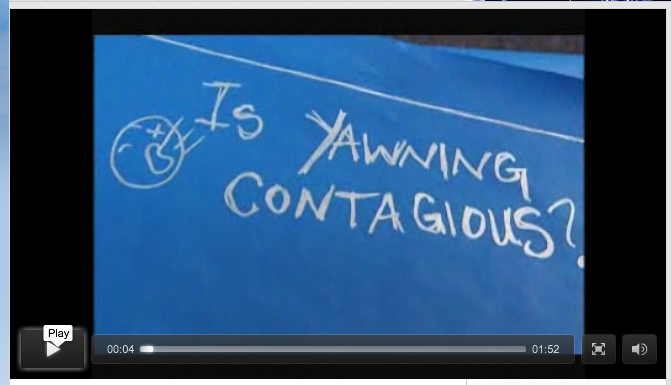
\includegraphics[width=0.7\textwidth]{figures/mythbusters}\\
\end{center}

\ct{\webURL{http://www.discovery.com/tv-shows/mythbusters/videos/is-yawning-contagious-minimyth.htm}}

\end{frame}


%%%%%%%%%%%%%%%%%%%%%%%%%%%%%%%%%%%

\begin{frame}
\frametitle{Experiment summary}

50 people were randomly assigned to two groups: 
\begin{itemize}
\item treatment: see someone yawn, $n = 34$
\item control: don't see someone yawn, $n = 16$
\end{itemize}

\begin{center}
\renewcommand\arraystretch{1.5}
\begin{tabular}{ l | c | c | c }
			& Treatment			& Control			& Total \\
\hline
Yawn		& 10				& 4				& 14 \\
Not Yawn		& 24				& 12				& 36 \\
\hline
Total			& 34				& 16				& 50 \\
\hline
\% Yawners	& \soln{\onslide<2->{$\frac{10}{34} = 0.29$}}	& \soln{\onslide<3->{$\frac{4}{16} = 0.25$}}	& 
\end{tabular}
\end{center}

\onslide<4->{

\disc{Based on the proportions we calculated, do you think yawning is really contagious, i.e. are seeing someone yawn and yawning dependent?}

}

\end{frame}

%%%%%%%%%%%%%%%%%%%%%%%%%%%%%%%%%%%

\begin{frame}
\frametitle{Dependence, or another possible explanation?}

\begin{itemize}

\item The observed differences might suggest that yawning is contagious, i.e. seeing someone yawn and yawning are dependent

\pause

\item But the differences are small enough that we might wonder if they might simple be \hl{due to chance}

\pause

\item Perhaps if we were to repeat the experiment, we would see slightly different results

\pause

\item So we will do just that - well, somewhat - and see what happens

\pause

\item Instead of actually conducting the experiment many times, we will \hl{simulate} our results

\end{itemize}

\end{frame}

%%%%%%%%%%%%%%%%%%%%%%%%%%%%%%%%%%%%

\subsection{Competing claims}

%%%%%%%%%%%%%%%%%%%%%%%%%%%%%%%%%%%%%

\begin{frame}
\frametitle{Two competing claims}

\begin{enumerate}

\item ``There is nothing going on." \\
Seeing someone yawn and yawning are \hl{independent}, observed difference in proportions of yawners in the treatment and control is simply due to chance. $\rightarrow$ \hl{Null hypothesis}

\pause

\item ``There is something going on." \\
Seeing someone yawn and yawning are \hl{dependent}, observed difference in proportions of yawners in the treatment and control is not due to chance. $\rightarrow$ \hl{Alternative hypothesis}

\end{enumerate}

\end{frame}

%%%%%%%%%%%%%%%%%%%%%%%%%%%%%%%%%%%%

\begin{frame}
\frametitle{A trial as a hypothesis test}

\begin{center}
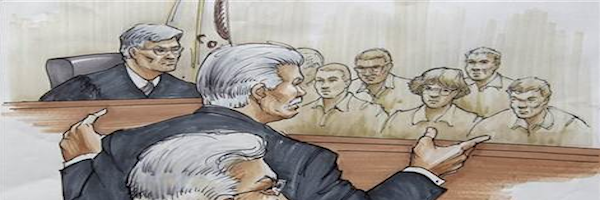
\includegraphics[width=\textwidth]{figures/trial}
\end{center}

\begin{itemize}

\item $H_0$: Defendant is innocent 

\item $H_A$: Defendant is guilty

\item Present the evidence: collect data.

\item Judge the evidence: ``Could these data plausibly have happened by chance if the null hypothesis were true?"

\item Make a decision: ``How unlikely is unlikely?"

\end{itemize}

\end{frame}

%%%%%%%%%%%%%%%%%%%%%%%%%%%%%%%%%%%%%

\subsection{Testing via simulation}

%%%%%%%%%%%%%%%%%%%%%%%%%%%%%%%%%%%%%

\begin{frame}
\frametitle{Simulation setup}

\begin{itemize}

\item A regular deck of cards is comprised of 52 cards: 4 aces, 4 of numbers 2-10, 4 jacks, 
4 queens, and 4 kings.

\item Take out two aces from the deck of cards and set them aside.

\item The remaining 50 playing cards to represent each participant in the study:
\begin{itemize}
\item 14 face cards (including the 2 aces) represent the people who yawn.
\item 36 non-face cards represent the people who don't yawn.
\end{itemize}

\end{itemize}

\vfill

[DEMO: Watch me go through the activity before you start it in your teams.]

\end{frame}

%%%%%%%%%%%%%%%%%%%%%%%%%%%%%%%%%%%

\begin{frame}
\frametitle{}

\activity{Running the simulation}{
\begin{enumerate}
\item Shuffle the 50 cards at least 7 times to ensure that the cards counted out are from a random process
\item Divide the cards into two decks:
\begin{itemize}
\item deck 1: 16 cards $\rightarrow$ control
\item deck 2: 34 cards $\rightarrow$ treatment
\end{itemize}
\item Count the number of face cards (yawners) in each deck
\item Calculate the difference in proportions of yawners \red{(treatment - control)}, and submit this value 
using your clicker (value must be between 0 and 1) - \textbf{only one submission per team per simulation}
\item Repeat steps (1) - (4) many times
\end{enumerate}
}

\vfill

\ct{Why shuffle 7 times: \webURL{http://www.dartmouth.edu/~chance/course/topics/winning_number.html}}

\end{frame}

%%%%%%%%%%%%%%%%%%%%%%%%%%%%%%%%%%%

\subsection{Checking for independence}

\begin{frame}

\clicker{Do the simulation results suggest that yawning is contagious, i.e. does seeing someone yawn and yawning appear to be dependent? \\
(Hint: In the actual data the difference was 0.04, does this appear to be an unusual observation for the chance model?)}

\begin{multicols}{2}
\begin{enumerate}[(a)]
\item Yes
\item No
\end{enumerate}
\end{multicols}

\end{frame}

%%%%%%%%%%%%%%%%%%%%%%%%%%%%%%%%%%%%

\section{Case study: Tapping on caffeine}

%%%%%%%%%%%%%%%%%%%%%%%%%%%%%%%%%%%%

\begin{frame}
\frametitle{Tapping on caffeine}

\begin{itemize}

\item In a double-blind experiment a sample of male college students were asked to tap their fingers at a rapid rate. 

\item The sample was then divided at random into two groups of 10 students each. 

\item Each student drank the equivalent of about two cups of coffee, which included about 200 mg of caffeine for the students in one group but was decaffeinated coffee for the second group. 

\item After a two hour period, each student was tested to measure finger tapping rate (taps per minute). 

\end{itemize}

\end{frame}

%%%%%%%%%%%%%%%%%%%%%%%%%%%%%%%%%%%%

\begin{frame}
\frametitle{Data}

\begin{center}
\begin{tabular}{rrl}
  \hline
 & Taps & Group \\ 
  \hline
1 & 246 & Caffeine \\ 
  2 & 248 & Caffeine \\ 
  3 & 250 & Caffeine \\ 
  4 & 252 & Caffeine \\ 
  5 & 248 & Caffeine \\ 
  6 & 250 & Caffeine \\ 
$\cdots$ && \\
  16 & 248 & NoCaffeine \\ 
  17 & 242 & NoCaffeine \\ 
  18 & 244 & NoCaffeine \\ 
  19 & 246 & NoCaffeine \\ 
  20 & 242 & NoCaffeine \\ 
   \hline
\end{tabular}
\end{center}

\end{frame}

%%%%%%%%%%%%%%%%%%%%%%%%%%%%%%%%%%%%

\begin{frame}
\frametitle{}

\clicker{What type of plot would be useful to visualize the distributions of tapping rate in the caffeine and no caffeine groups.}

\begin{enumerate}[(a)]
\item Bar plot
\item Mosaic plot
\item Pie chart
\item \solnMult{Side-by-side box plots}
\item Single box plot
\end{enumerate}

\end{frame}

%%%%%%%%%%%%%%%%%%%%%%%%%%%%%%%%%%%%

\begin{frame}
\frametitle{Exploratory data analysis}

\twocol{0.4}{0.6}{
\disc{Compare the distributions of tapping rates in the caffeine and no caffeine groups.}
}
{
\begin{center}
{\footnotesize
\begin{tabular}{l | c | c | c}
\hline
		& Caffeine	& No Caffeine	& Difference \\
\hline
mean	&  248.3		& 244.8 		& 3.5 \\
SD		& 2.21		& 2.39 		& -0.18 \\
median	& 248		& 245 		& 3 \\
IQR		& 3.5			& 4.25		& -0.75 \\
\hline
\end{tabular}
}
\end{center}
}

\vspace{-1cm}

\begin{center}
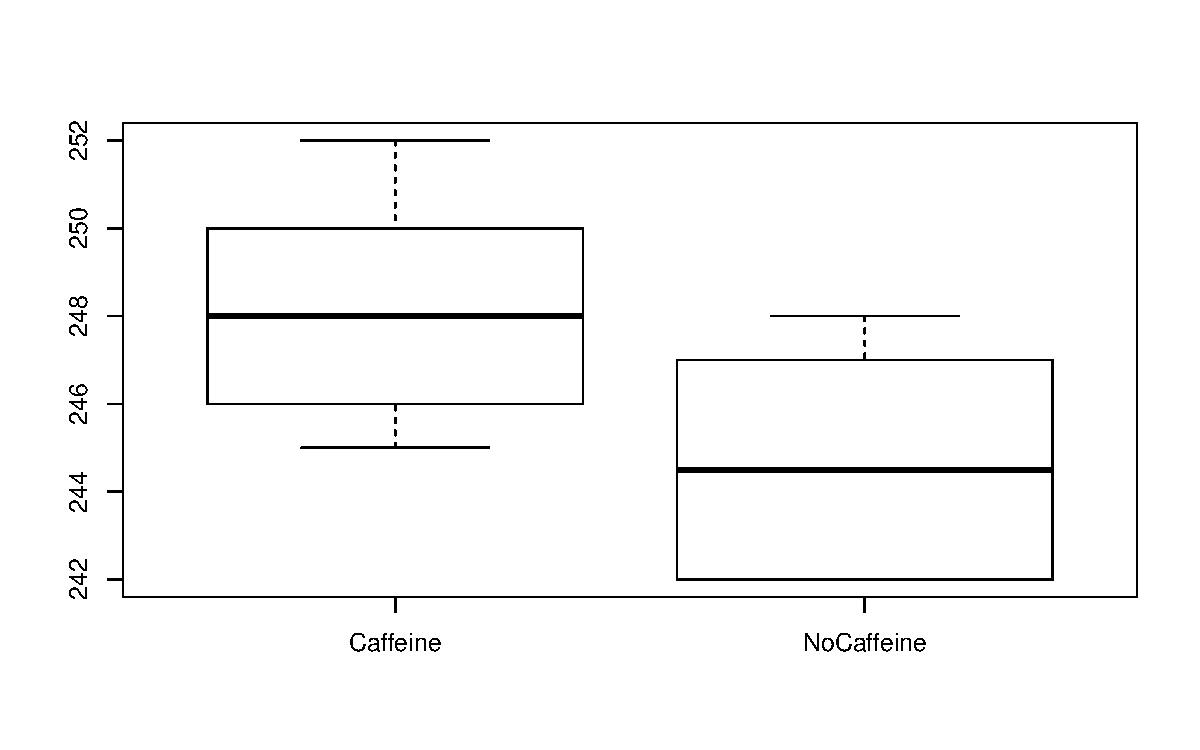
\includegraphics[width=0.85\textwidth]{figures/caffeine/caffeinetaps_box.pdf}
\end{center}

\end{frame}

%%%%%%%%%%%%%%%%%%%%%%%%%%%%%%%%%%%%

\begin{frame}
\frametitle{}

\clicker{We are interested in finding out if caffeine increases tapping rate. Which of the following are the correct set of hypotheses?}

\begin{enumerate}[(a)]

\item $H_0: \mu_{caff} = \mu_{no~caff}$ \\
$H_A: \mu_{caff} < \mu_{no~caff}$

\item \solnMult{$H_0: \mu_{caff} = \mu_{no~caff}$ \\
$H_A: \mu_{caff} > \mu_{no~caff}$}

\item $H_0: \bar{x}_{caff} = \bar{x}_{no~caff}$ \\
$H_A: \bar{x}_{caff} > \bar{x}_{no~caff}$

\item $H_0: \mu_{caff} > \mu_{no~caff}$ \\
$H_A: \mu_{caff} = \mu_{no~caff}$

\item $H_0: \mu_{caff} = \mu_{no~caff}$ \\
$H_A: \mu_{caff} \ne \mu_{no~caff}$

\end{enumerate}

\end{frame}

%%%%%%%%%%%%%%%%%%%%%%%%%%%%%%%%%%%%

\begin{frame}
\frametitle{Simulation scheme}

\begin{itemize}

\item On 20 index cards write the tapping rate of each subject in the study.

\item Shuffle the cards and divide them into two stacks of 10 cards each, label one stack ``caffeine" and the other stack ``no caffeine".

\item Calculate the average tapping rates in the two simulated groups, and record the difference on a dot plot.

\item Repeat steps (2) and (3) many times to build a \hl{randomization distribution}.

\end{itemize}

\end{frame}

%%%%%%%%%%%%%%%%%%%%%%%%%%%%%%%%%%%%

\begin{frame}
\frametitle{Making a decision}

\vspace{-0.5cm}

\disc{Below is a randomization distribution of 100 simulated differences in means ($\bar{x}_c - \bar{x}_{nc}$). Calculate the p-value for the hypothesis test evaluating whether caffeine \underline{increases} average tapping rate.
\begin{center}
{\footnotesize
\begin{tabular}{l | c | c | c}
\hline
		& Caffeine	& No Caffeine	& Difference \\
\hline
mean	&  248.3		& 244.8 		& 3.5 \\
\hline
\end{tabular}
}
\end{center}
}

\begin{center}
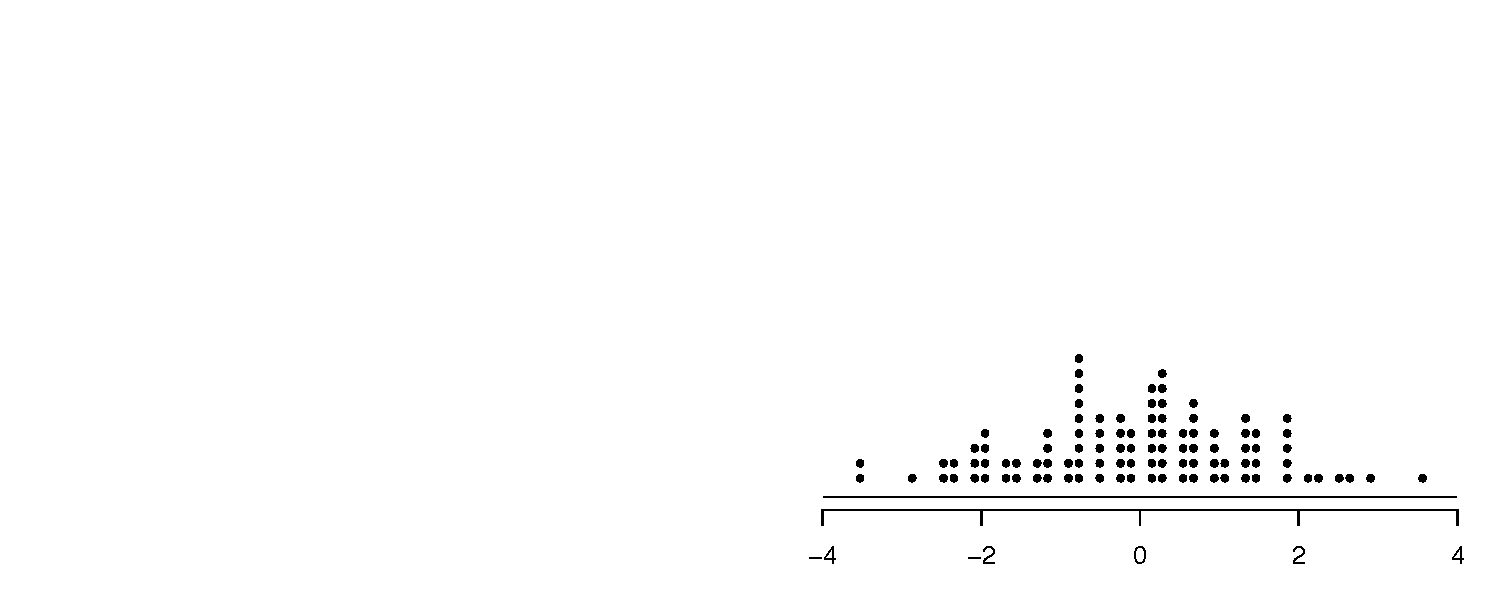
\includegraphics[width=0.9\textwidth]{figures/caffeine/caffeinetaps_mean_ht.pdf}
\end{center}

\pause

\soln{1/100 = 0.01}

\end{frame}

%%%%%%%%%%%%%%%%%%%%%%%%%%%%%%%%%%%%

\begin{frame}
\frametitle{Testing for the median}

\disc{Describe how could we use the same approach to test whether the \underline{median} tapping rate is higher for the caffeine group?}

\soln{\only<2>{Use the same simulation scheme but record the difference between the medians instead of the means, and calculate the p-value as the proportion of simulations where the simulated difference in medians is at least 3.
}}

\end{frame}

%%%%%%%%%%%%%%%%%%%%%%%%%%%%%%%%%%%%

\begin{frame}
\frametitle{Testing for the median (cont.)}

\vspace{-0.5cm}

\disc{Below is a randomization distribution of 100 simulated differences in medians ($med_c - med_{nc}$). Do the data provide convincing evidence that caffeine increases \underline{median} tapping rate?
\begin{center}
{\footnotesize
\begin{tabular}{l | c | c | c}
\hline
		& Caffeine	& No Caffeine	& Difference \\
\hline
median	& 248		& 245 		& 3 \\
\hline
\end{tabular}
}
\end{center}
}

\begin{center}
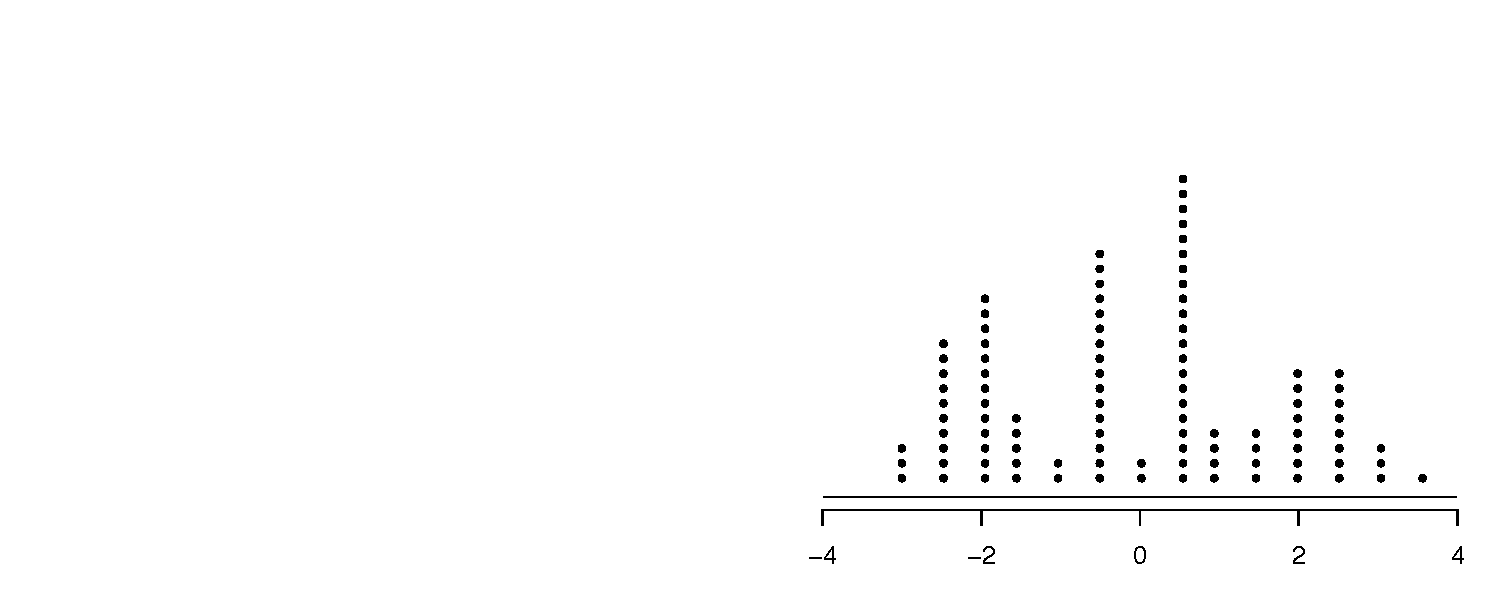
\includegraphics[width=0.65\textwidth]{figures/caffeine/caffeinetaps_median_ht.pdf}
\end{center}

\end{frame}

%%%%%%%%%%%%%%%%%%%%%%%%%%%%%%%%%%%%

\section{Application exercise}

%%%%%%%%%%%%%%%%%%%%%%%%%%%%%%%%%%%

\begin{frame}
\frametitle{}

\vfill

\app{1.4 Randomization testing}{$\:$\\ See the course website for instructions. \\$\:$}

\vfill

\end{frame}

%%%%%%%%%%%%%%%%%%%%%%%%%%%%%%%%%%%

\end{document}